\documentclass{beamer}\usepackage[]{graphicx}\usepackage[]{color}
%% maxwidth is the original width if it is less than linewidth
%% otherwise use linewidth (to make sure the graphics do not exceed the margin)
\makeatletter
\def\maxwidth{ %
  \ifdim\Gin@nat@width>\linewidth
    \linewidth
  \else
    \Gin@nat@width
  \fi
}
\makeatother

\definecolor{fgcolor}{rgb}{0.345, 0.345, 0.345}
\newcommand{\hlnum}[1]{\textcolor[rgb]{0.686,0.059,0.569}{#1}}%
\newcommand{\hlstr}[1]{\textcolor[rgb]{0.192,0.494,0.8}{#1}}%
\newcommand{\hlcom}[1]{\textcolor[rgb]{0.678,0.584,0.686}{\textit{#1}}}%
\newcommand{\hlopt}[1]{\textcolor[rgb]{0,0,0}{#1}}%
\newcommand{\hlstd}[1]{\textcolor[rgb]{0.345,0.345,0.345}{#1}}%
\newcommand{\hlkwa}[1]{\textcolor[rgb]{0.161,0.373,0.58}{\textbf{#1}}}%
\newcommand{\hlkwb}[1]{\textcolor[rgb]{0.69,0.353,0.396}{#1}}%
\newcommand{\hlkwc}[1]{\textcolor[rgb]{0.333,0.667,0.333}{#1}}%
\newcommand{\hlkwd}[1]{\textcolor[rgb]{0.737,0.353,0.396}{\textbf{#1}}}%
\let\hlipl\hlkwb

\usepackage{framed}
\makeatletter
\newenvironment{kframe}{%
 \def\at@end@of@kframe{}%
 \ifinner\ifhmode%
  \def\at@end@of@kframe{\end{minipage}}%
  \begin{minipage}{\columnwidth}%
 \fi\fi%
 \def\FrameCommand##1{\hskip\@totalleftmargin \hskip-\fboxsep
 \colorbox{shadecolor}{##1}\hskip-\fboxsep
     % There is no \\@totalrightmargin, so:
     \hskip-\linewidth \hskip-\@totalleftmargin \hskip\columnwidth}%
 \MakeFramed {\advance\hsize-\width
   \@totalleftmargin\z@ \linewidth\hsize
   \@setminipage}}%
 {\par\unskip\endMakeFramed%
 \at@end@of@kframe}
\makeatother

\definecolor{shadecolor}{rgb}{.97, .97, .97}
\definecolor{messagecolor}{rgb}{0, 0, 0}
\definecolor{warningcolor}{rgb}{1, 0, 1}
\definecolor{errorcolor}{rgb}{1, 0, 0}
\newenvironment{knitrout}{}{} % an empty environment to be redefined in TeX

\usepackage{alltt}
\usetheme{metropolis}
\usepackage[utf8]{inputenc}
\usepackage{amsfonts}
\usepackage{amsmath}
\usepackage{natbib}
\usepackage{graphicx}
\usepackage{array,booktabs,tabularx}
\usepackage{epstopdf}
\usepackage{colortbl, xcolor}


\title{dpcReport: web server and software suite for unified analysis of digital PCRs and digital assays }
\date{}
\author{\scriptsize{Micha\l{} Burdukiewicz\inst{1}, 
Jim Huggett\inst{2},
Alexandra Whale\inst{2},
Piotr Sobczyk\inst{3}, 
Pawe\l{} Mackiewicz\inst{1},
Andrej-Nikolai Spiess\inst{3},
Peter Schierack\inst{5},
and Stefan R\"{o}diger\inst{5}}}

\institute{\tiny{\textsuperscript{1}University of Wroc\l{}aw, Department of Genomics, 

\textsuperscript{2}Molecular and Cell Biology Team, LGC, Teddington, United Kingdom,

\textsuperscript{3}Wroc\l{}aw University of Science and Technology, Faculty of Pure and Applied Mathematics,

\textsuperscript{4}University Medical Center Hamburg-Eppendorf, Hamburg, Germany,

\textsuperscript{5}Brandenburg University of Technology Cottbus-Senftenberg, Institute of Biotechnology 
}}
\IfFileExists{upquote.sty}{\usepackage{upquote}}{}
\begin{document}
  \maketitle
  
  \tableofcontents
  
  \section{dPCR software}
  
  \begin{frame}{}

  
% every rapidly emergining technique is accompanied by influx of the software
Words, words

\end{frame}
  
\section{Aim} 

\begin{frame}{Aim}

Create framework for dPCR data analysis:
\begin{itemize}[<+(1)->]
\item tailored for the most common tasks, 
%(comparison of multiple experiments and quality control),
\item unified,
\item reproducible.
\end{itemize}

\end{frame}


\section{Reproducibility}

\begin{frame}{Reproducibility}

Scientific software supports reproducibility, otherwise it is not scientific.

A report must contain enough information to allow the full reproduction of the conducted analysis.

\end{frame}


\begin{frame}{Reports}
\begin{figure} 
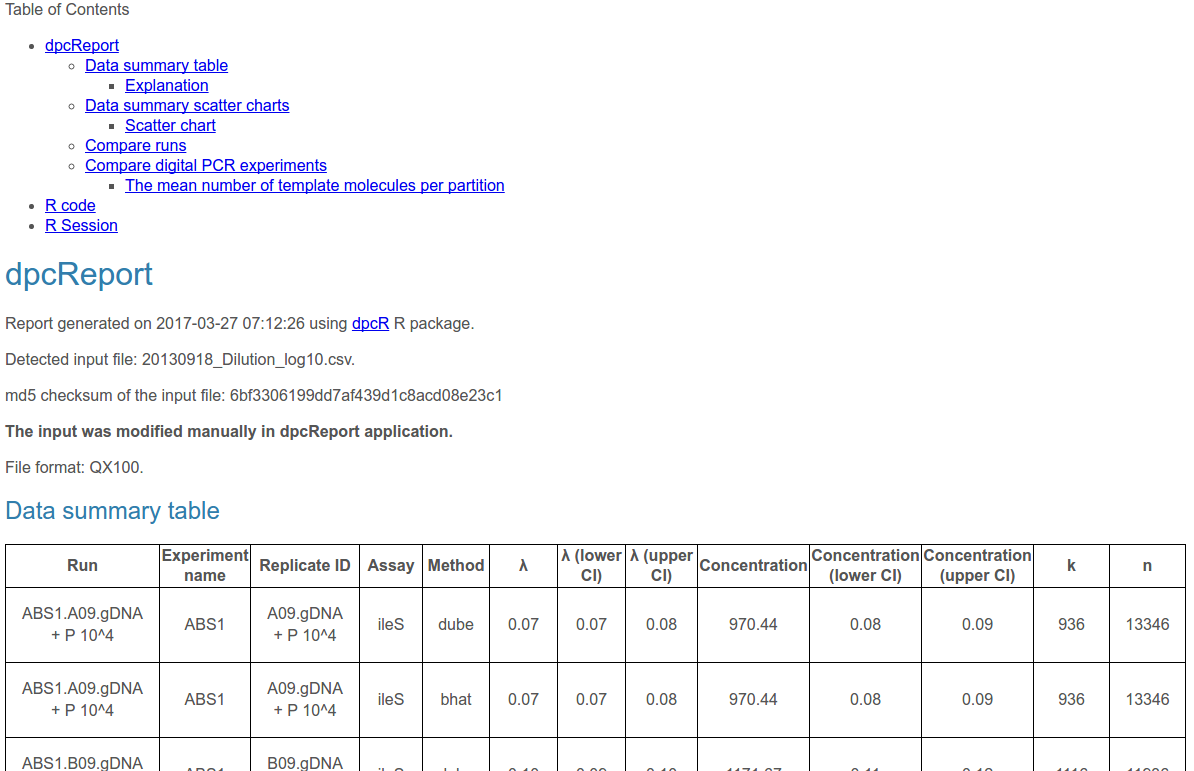
\includegraphics[width=0.95\textwidth]{static_figure/dcpReport_reprod1.png}
\end{figure}
\end{frame}


\begin{frame}{Date and time}
\begin{figure} 
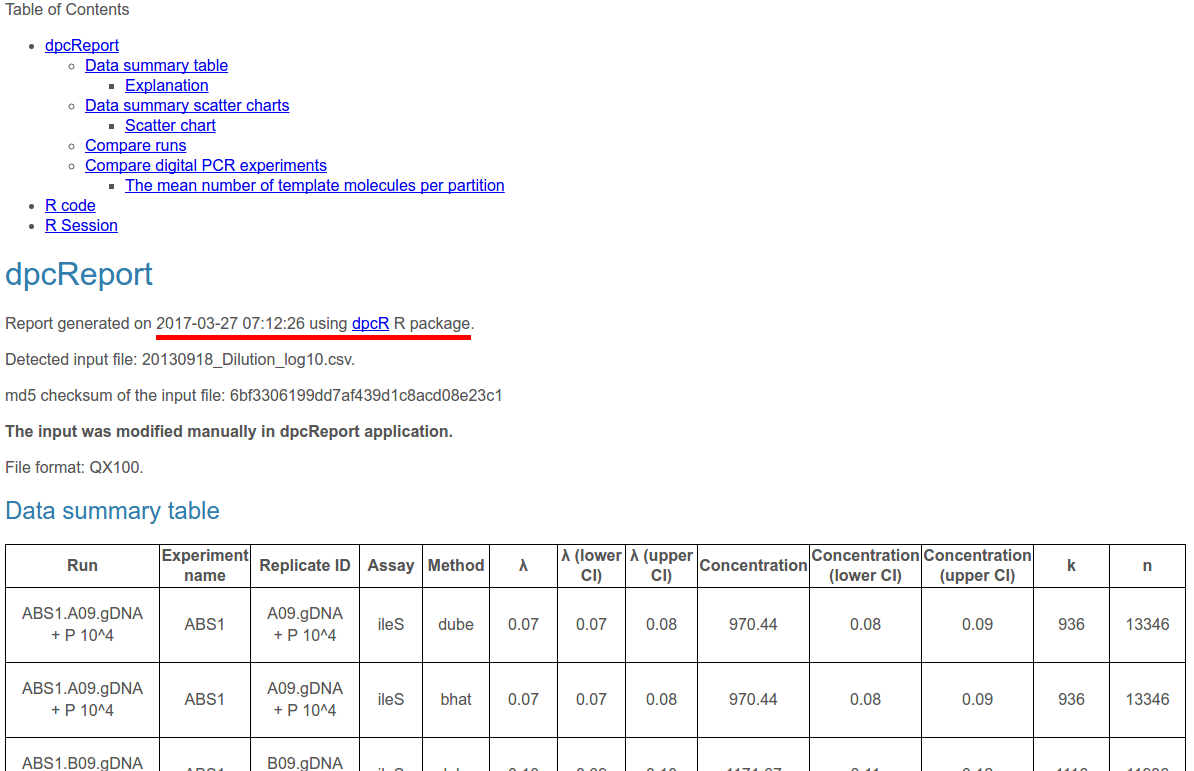
\includegraphics[width=0.95\textwidth]{static_figure/dcpReport_reprod2.png}
\end{figure}
\end{frame}


\begin{frame}{Input file name}
\begin{figure} 
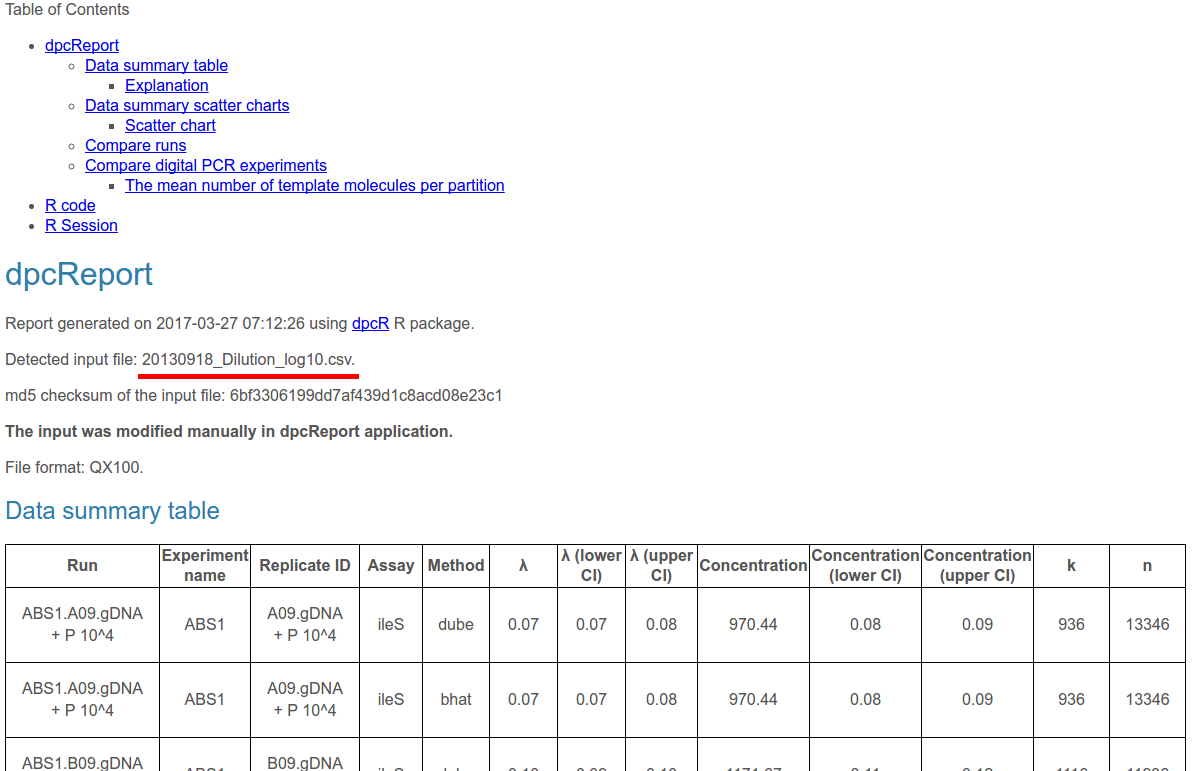
\includegraphics[width=0.95\textwidth]{static_figure/dcpReport_reprod3.png}
\end{figure}
\end{frame}


\begin{frame}{Input file checksum}
\begin{figure} 
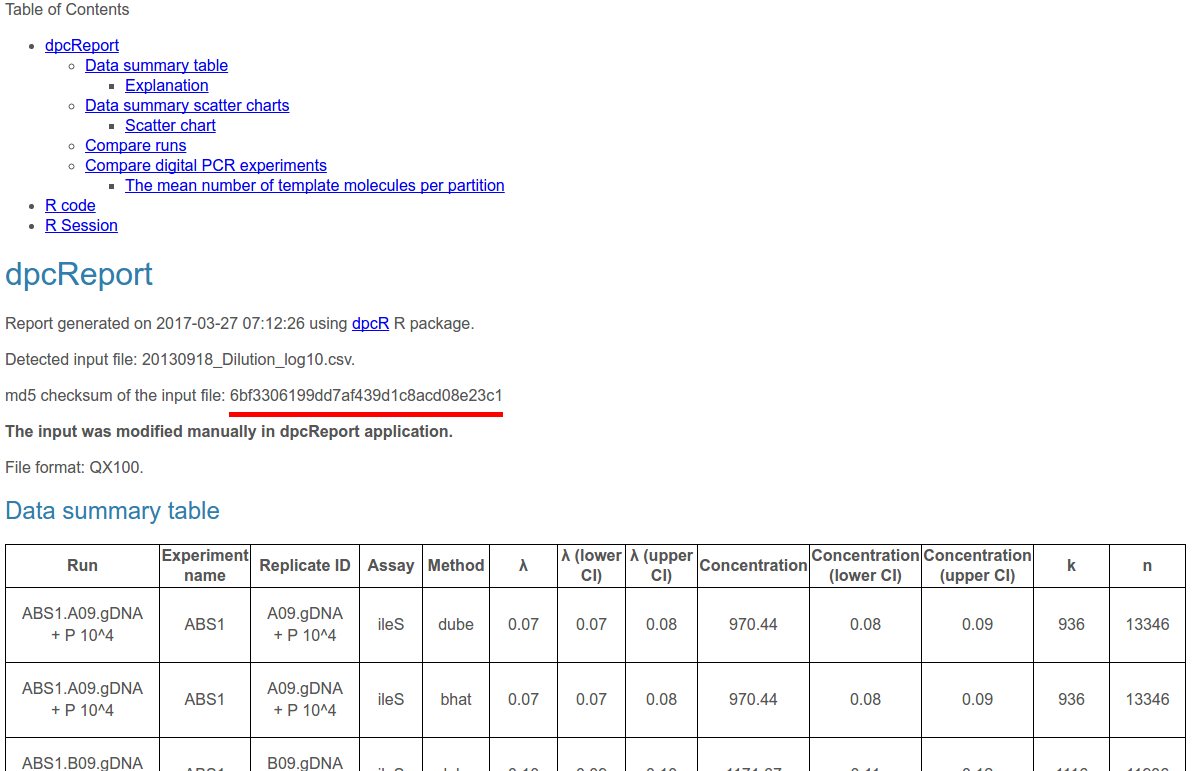
\includegraphics[width=0.95\textwidth]{static_figure/dcpReport_reprod4.png}
\end{figure}

Changes in case of the manual alteration of the input file.

\end{frame}


\begin{frame}{Manual alterations inside dpcReport}
\begin{figure} 
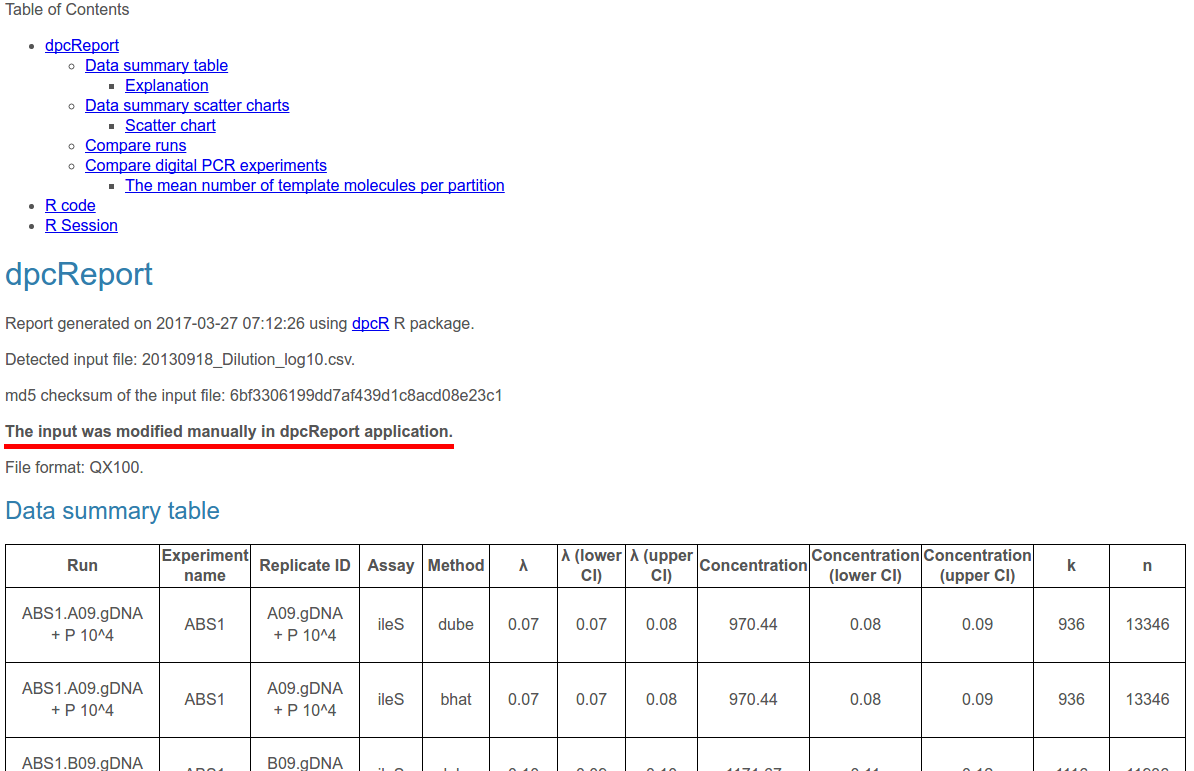
\includegraphics[width=0.95\textwidth]{static_figure/dcpReport_reprod5.png}
\end{figure}
\end{frame}


\begin{frame}{R Session}
\begin{figure} 
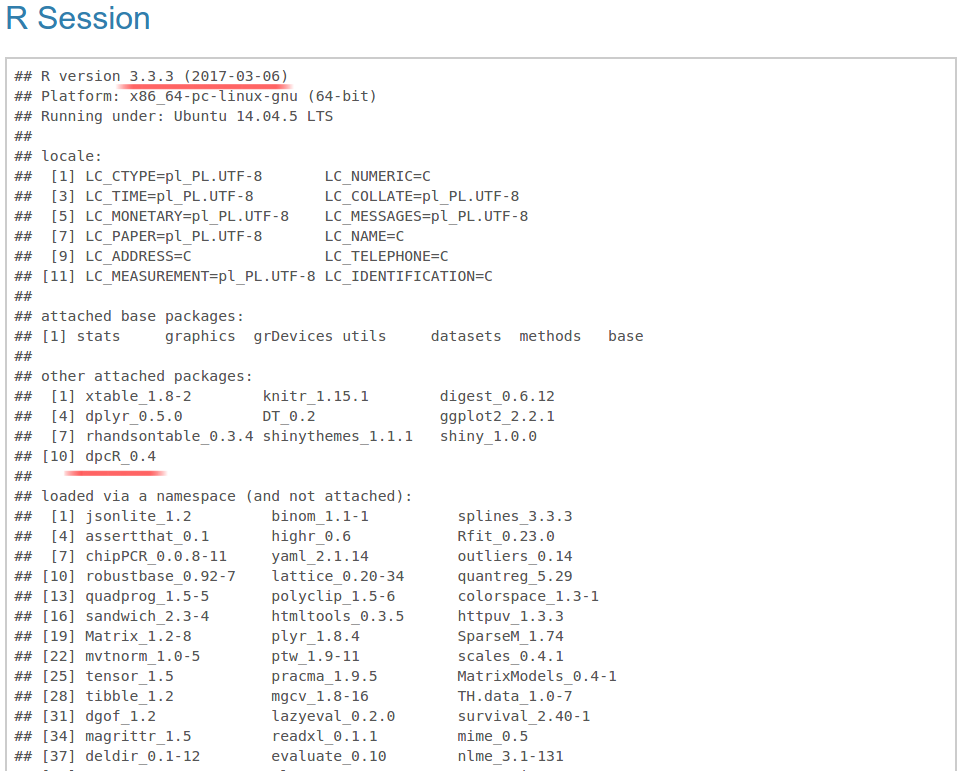
\includegraphics[width=0.95\textwidth]{static_figure/dcpReport_reprod6.png}
\end{figure}
\end{frame}


\begin{frame}{Reproducibility of the workflow}

An analysis conducted in a GUI-based software, as \textit{dpcReport}, is more challenging to reproduce.

dpcReport exports all steps of the analysis, including parameters adjusted manually by the user, in form of the \textbf{R} code that recreates the whole workflow.

\end{frame}

\begin{frame}{Reproducibility of the workflow}
\begin{figure} 
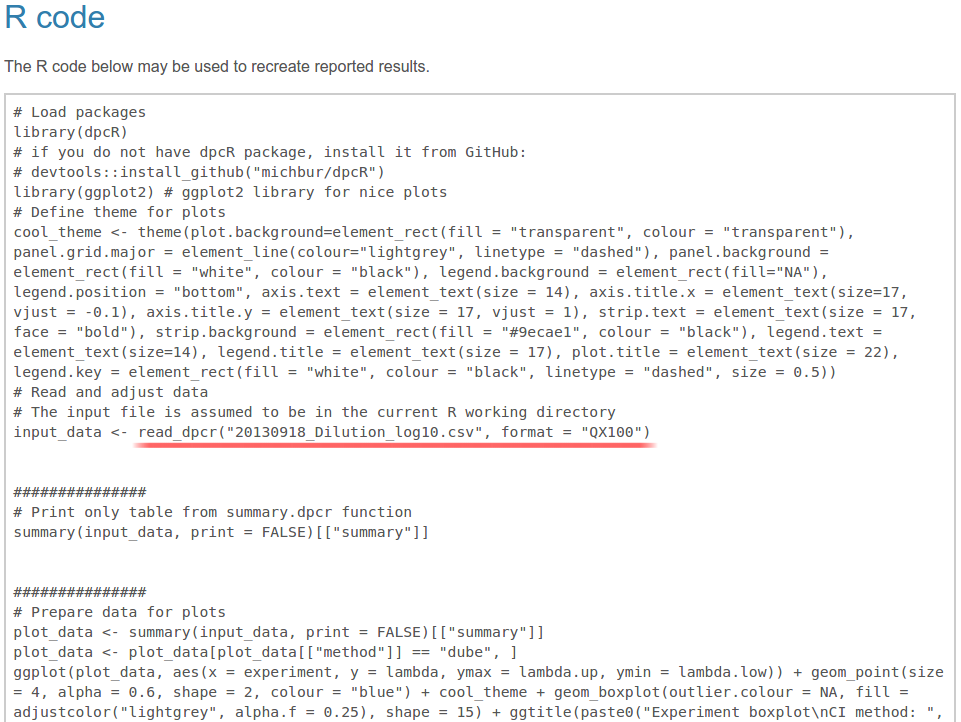
\includegraphics[width=0.95\textwidth]{static_figure/dcpReport_reprod7.png}
\end{figure}
\end{frame}


\begin{frame}{Summary}
\textit{dpcReport} is the integrted environment for the analysis of dPCR data.
\end{frame}


\begin{frame}{Availability}

Web server:
\url{www.smorfland.uni.wroc.pl/shiny/dpcReport}

R package (including your local instance of dpcReport):
\url{www.github.com/michbur/dpcR}

\end{frame}

\begin{frame}{Acknowledgements and funding}

This research was partially funded by the KNOW Consortium and National Science Center (2015/17/N/NZ2/01845).

\small{
\begin{itemize}
\item Małgorzata Kotulska.
\item Paweł Mackiewicz,
\item Stefan R\"{o}diger,
\item \textbf{biogram} package (\url{https://cran.r-project.org/package=biogram}):
\begin{itemize}
\small
\item Piotr Sobczyk,
\item Chris Lauber,
\end{itemize}

\item \textbf{AmyLoad} database (\url{comprec-lin.iiar.pwr.edu.pl/amyload}):
\begin{itemize}
\small
\item Paweł Woźniak,
\end{itemize}
\end{itemize}
}

\end{frame}



\begin{frame}[allowframebreaks]
        \frametitle{References}
  \bibliographystyle{apalike}
  \bibliography{references}
\end{frame}  


\end{document}
